\documentclass{standalone}
\usepackage{tikz}
\usepackage{tikz-cd}
\usepackage{tikz-3dplot}
\usepackage{pgfplots}
\usepackage{pgffor} % For \foreach loop
\pgfplotsset{compat=newest} % Adjust to your version of pgfplots
\def\Circlearrowleft{\ensuremath{%
		\rotatebox[origin=c]{180}{$\circlearrowleft$}}}
\def\Circlearrowright{\ensuremath{%
		\rotatebox[origin=c]{180}{$\circlearrowright$}}}
\def\CircleArrowleft{\ensuremath{%
		\reflectbox{\rotatebox[origin=c]{180}{$\circlearrowleft$}}}}
\def\CircleArrowright{\ensuremath{%
		\reflectbox{\rotatebox[origin=c]{180}{$\circlearrowright$}}}}
\usetikzlibrary{
	3d, % For 3D drawing
	angles,
	arrows,
	arrows.meta,
	backgrounds,
	bending,
	calc,
	decorations.pathmorphing,
	decorations.pathreplacing,
	decorations.markings,
	fit,
	matrix,
	patterns,
	patterns.meta,
	positioning,
	quotes,
	shadows,
	shapes,
	shapes.geometric
}

\begin{document}
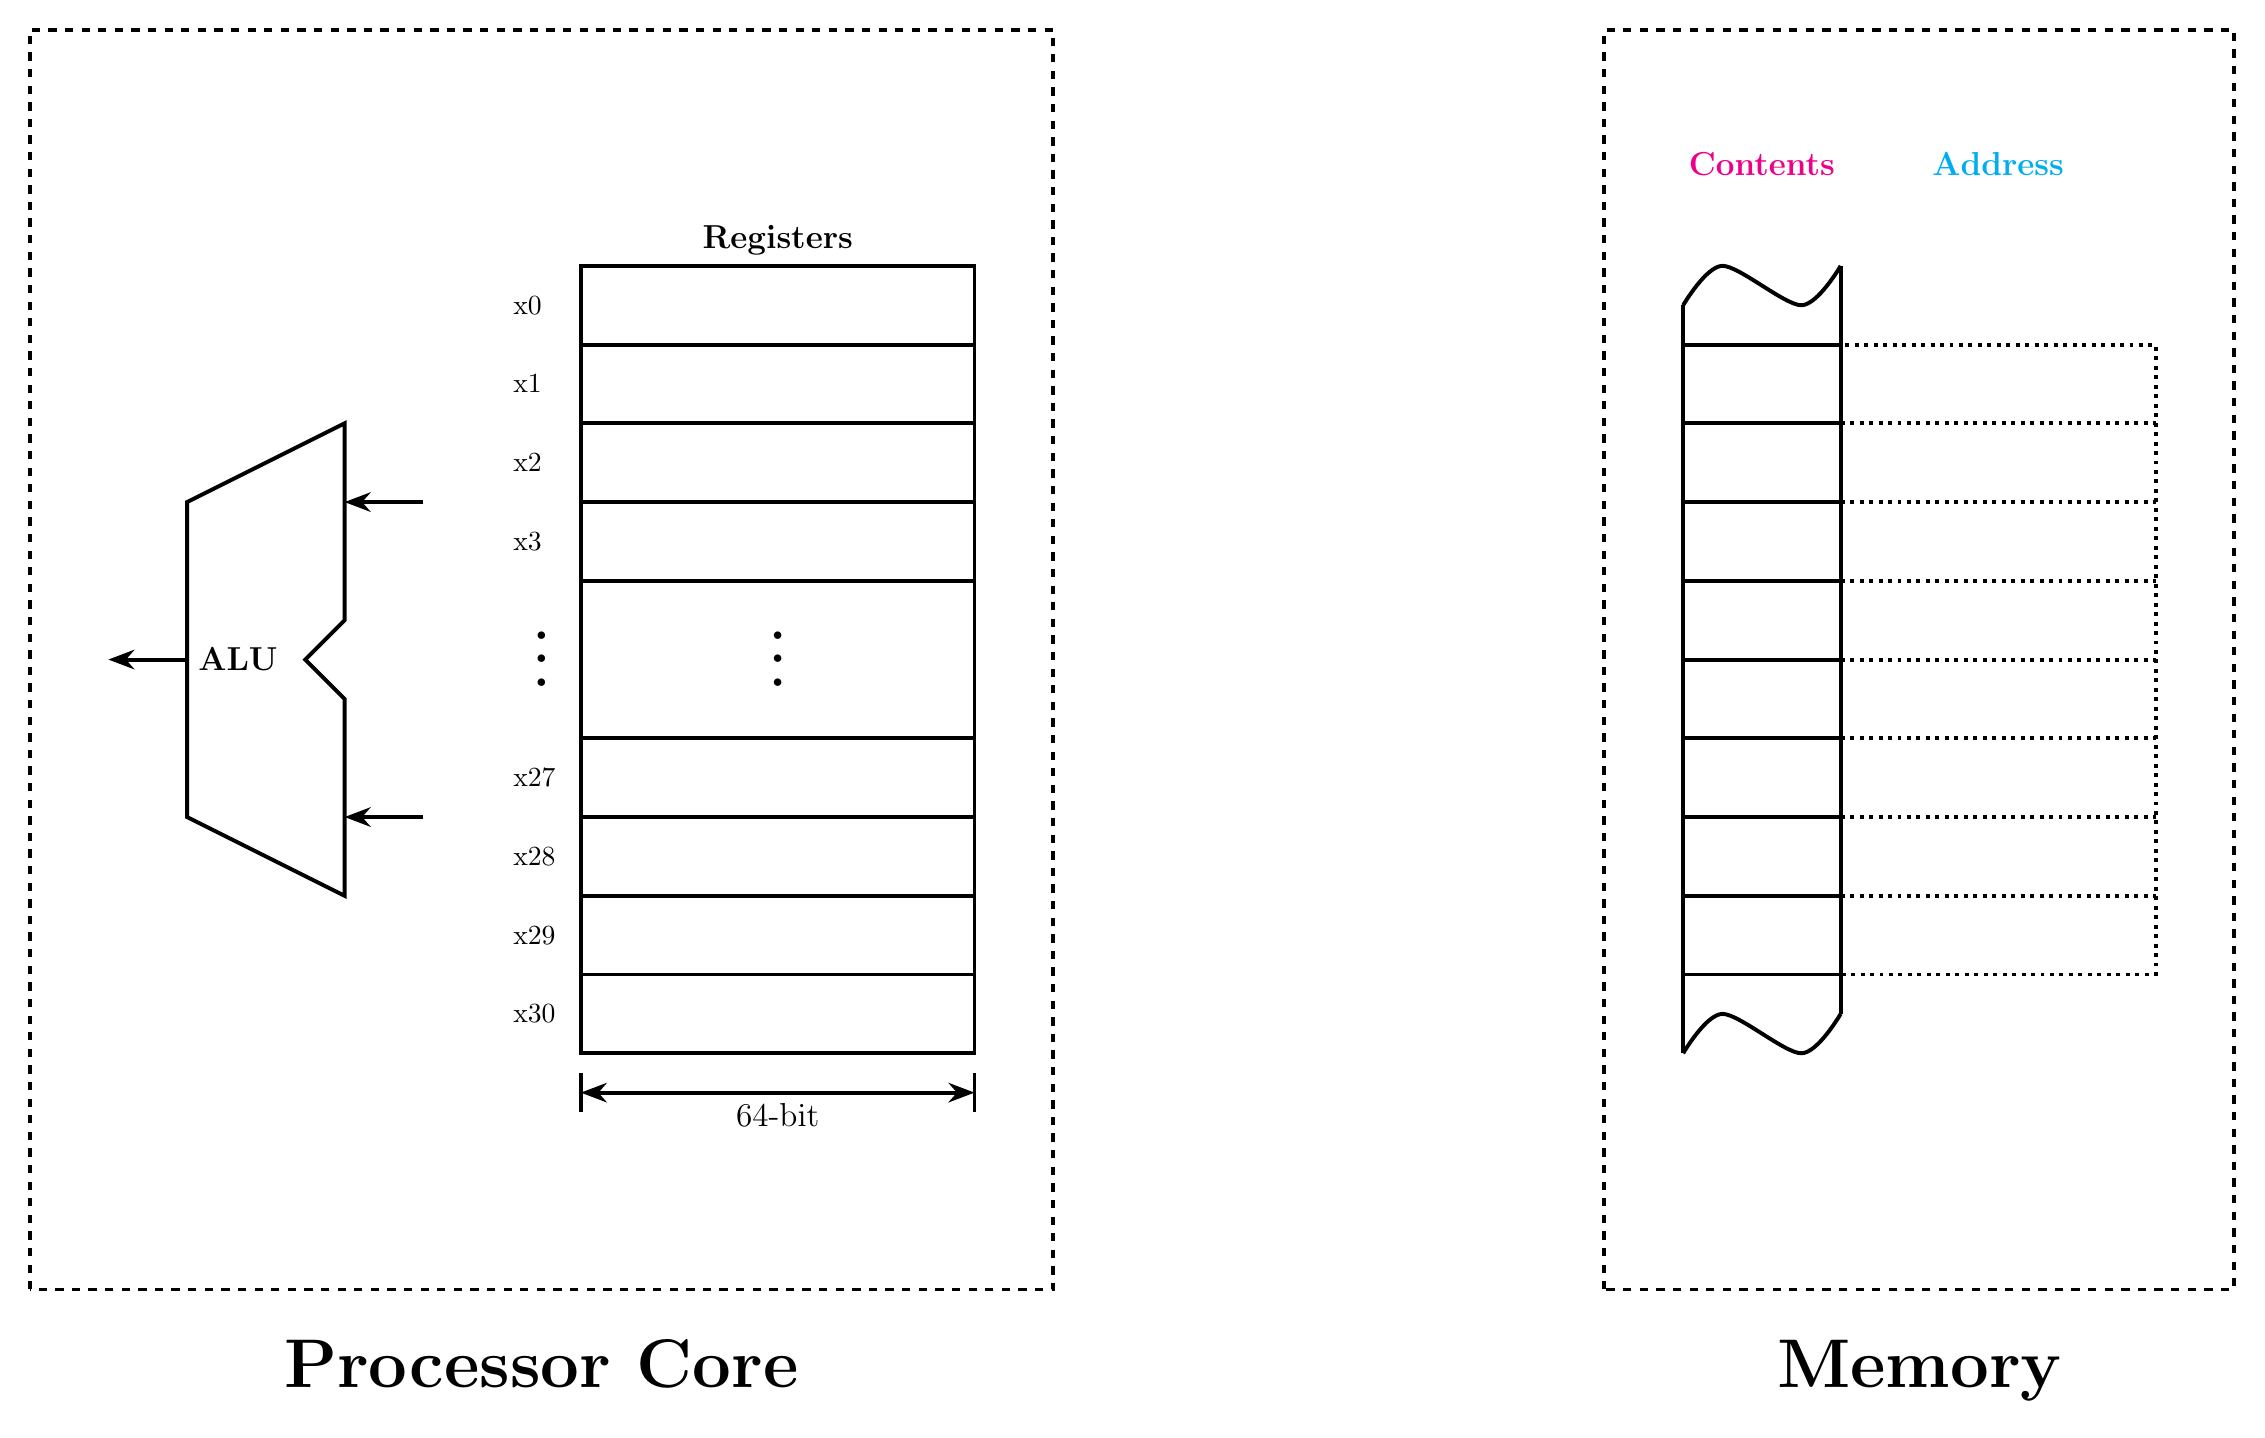
\begin{tikzpicture}[>=Stealth, line width=.5mm]
	\def \x{15}
	\def \y{10}
%	\draw[very thin,color=gray!15,step=.5] (-\x,-\y) grid (\x,\y);
%	
%	\foreach \i in {-\x,...,-2,-1,1,2,...,\x}
%	\draw[gray] (\i,.1)--(\i,-.1) node[below] {$\i$};%x-axis
%	\foreach \i in {-\y,-1,1,1,\y}
%	\draw[gray] (.1,\i)--(-.1,\i) node[left] {$\i$};%y-axis
	
	\begin{scope}[xshift=-2cm]
	% ALU Section (at x = -2)
	\draw[] (-10, -2) -- (-8, -3) -- (-8, -.5) -- (-8.5, 0) -- (-8, .5) -- (-8, 3) -- (-10, 2) -- cycle node[midway, right] {\large\bf ALU};
	\draw[->] (-10, 0) to (-11, 0);
	\draw[->] (-7, 2) to (-8, 2);
	\draw[->] (-7, -2) to (-8, -2);

	% Registers section (left side)
	\node[above] at (-2.5, 5) {\large\bf Registers};
	\draw[] (-5, -5) rectangle (0, 5); % Outer box
	\foreach \i in {0, 1, 2, 3} {
		\node[anchor=west] at (-6, 4.5-\i) {x\i};
	}
	\foreach \i in {27, 28, 29, 30} {
		\node[anchor=west] at (-6, -1.5-\i+27) {x\i};
	}
	\node[align=center,scale=.7] at (-5.5, 0) {$\bullet$\\ $\bullet$\\ $\bullet$};
	\node[align=center,scale=.7] at (-2.5, 0) {$\bullet$\\ $\bullet$\\ $\bullet$};
	\foreach \i in {4,3,2,1} {
		\draw (-5,\i) -- (0, \i);
		\draw (-5,-\i) -- (0, -\i);
	}
	\draw[] (-5, -5.25) to (-5, -5.75);
	\draw[] (0, -5.25) to (0, -5.75);
	\draw[<->] (-5, -5.5) to (0, -5.5);
	\node[below] at (-2.5, -5.5) {\large $64$-bit};
	\draw[dashed] (-12, -8) rectangle (1, 8);
	\node[below] at (-5.5, -8.5) {\Huge\bf Processor Core};
	\end{scope}
	
	% Memory section (right side)
	\begin{scope}[xshift=7cm]
	\node[magenta, above] at (1, 6) {\large\bf Contents};
	\node[cyan, above] at (4, 6) {\large\bf Address};
	\draw[] (0, -4) rectangle (2, 4); % Outer box
	\draw[dotted] (2, -4) rectangle (6, 4); % Outer box
	\foreach \i in {3,2,1,0} {
		\draw (0,\i) -- (2, \i);
		\draw (0,-\i) -- (2, -\i);
	}
	\foreach \i in {3,2,1,0} {
		\draw[dotted] (2,\i) -- (6, \i);
		\draw[dotted] (2,-\i) -- (6, -\i);
	}
	\draw (0,4) to (0,4.5); \draw (2,4) to (2,5);
	\draw[smooth] plot coordinates {(0,4.5) (.5, 5) (1.5, 4.5) (2,5)};
	\draw (0,-4) to (0,-5); \draw (2,-4) to (2,-4.5);
	\draw[smooth] plot coordinates {(2,-4.5) (1.5, -5) (.5, -4.5) (0,-5)};
	\draw[dashed] (-1, -8) rectangle (7, 8);
	\node[below] at (3, -8.5) {\Huge\bf Memory};
	\end{scope}
\end{tikzpicture}
\end{document}
